\chapter{Artifact Development}

This chapter describes the development of the artifact, \texttt{ARKIVO.ART}, following the RQDD method introduced in the previous chapter.

\section{Plan Breakdown}

To answer a research question, one starts to plan what is required to answer the question, and then works backwards in incremental stages to where we are currently, leaving milestones (Miles) along the way, starting at 1 and going upwards as we get away from the goal. The analogy is that of a road, with each side-road marker showing how many miles we are away from a city, as we drive away from it.

We will start by trying to answer RQ1:

\vspace{0.5cm}

RQ1 - Can we determine which code-based HEN OBJKTs are networked?

\vspace{0.5cm}

We know that we can do this manually, by opening the OBJKT on a web browser and inspecting the network tab under the Developer Tools, to determine if there is any network activity to a domain or URL path that is outside of the OBJKT's IPFS URL. As an example we will use the artwork ``Adam'' by Raphaël de Courville\footnotemark[1], which we know to be a networked OBJKT.
As seen in \autoref{fig:devtools-net}, there is indeed a request to an external endpoint: \texttt{https\://api.hicdex.com/v1/graphql} initated by \texttt{sketch.js}, which is the p5js sketch that renders this artwork. The remaining 3 network requests are for local assets within the directory of the OBJKT, and hence not considered 'networking' as per our initial definition.

\footnotetext[1]{https://cache.teia.rocks/ipfs/QmbNtTu7k2E2UDYDQTyiVzV8rVbCU44hc9js1erKzeSogY/?\\creator=tz1hfuVWgcJ89ZE75ut9Qroi3y7GFJL5Lf2K\&viewer=\&objkt=230177}

\begin{figure}[h]
    \centering
    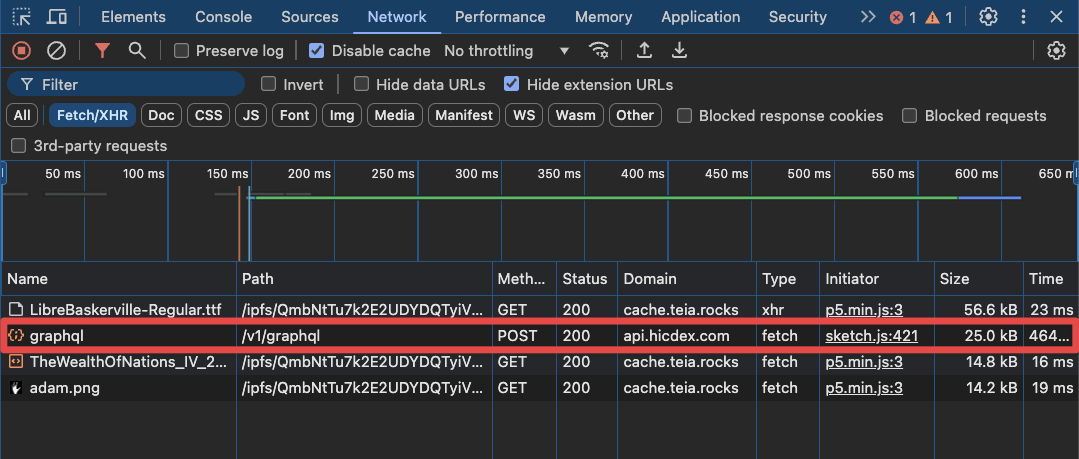
\includegraphics[width=\linewidth]{dev-tools-net.png}
    \caption[Developer Tools - Network Inspection]{Developer Tools - Network Inspection}
    \label{fig:devtools-net}
\end{figure}

Now that we established that we can identify a networked OBJKT manually, the next step is to do it programatically.

At this stage we can start to plan our Miles. The numbers will go up the further we get away from our goal.

Analysing the network traffic and determining if an OBJKT is networked is Mile 1.


For capturing the network traffic programatically we can use one of several headless browser automation solutions, which are normally used for automated website testing and web-scraping, like Playwright\footnotemark[2], Selenium\footnotemark[3], or Puppeteer\footnotemark[4]. For this work Playwright was selected. This is Mile 2.


\footnotetext[2]{https://playwright.dev/}
\footnotetext[3]{https://www.selenium.dev/}
\footnotetext[4]{https://pptr.dev/}

Although our Playwright instance could access the OBJKT asset directly from the Teia IPFS node, there are several reasons why it's not desirable to do so:

\begin{enumerate}
	\item introduces potential network latency which could affect the snapshot process adversely
	\item increases the bandwidth usage between teia and arkivo
	\item arkivo is supposed to archive these artworks anyway, including full copies of the assets
\end{enumerate}

For this reason the next step is to run our own IPFS node, so that we can fetch the OBJKTs locally, and pin them, which ensured it cannot be garbage collected by the node. This is Mile 3.

But this raises another question, which artworks to fetch? We need a way to discover and index all the OBJKTs that we are interested in investigating. This is Mile 4.

To discover the OBJKTs we can resort to existing indexers of the Tezos blockchain. There are 2 main options:

\begin{enumerate}
	\item TzKT API\footnotemark[5] - a generic indexer for the whole Tezos blockchain
	\item TezTok API\footnotemark[6] - an indexer specialised in Tezos NFTs
\end{enumerate}

\footnotetext[5]{https://tzkt.io/api}
\footnotetext[6]{https://www.teztok.com}

The TzKT API being generic, operates at a very low level, with endpoints that are closely related to the blockchain data, without abstraction layers.
TezTok, on the other hand, specialises in NFTs so it creates an abstraction layer that is easier to work with, since it is NFTs we are interested in discovering. For this reason TezTok was chosen.

Finally, we can move to the last stage, determining what search criteria to use when querying Teztok. This is Mile 5.

Here is a summary of the five Miles. We will write them in the reverse order, as now we are going back towards our goal.

\vspace{0.5cm}

\begin{table}[h]
\footnotesize
\centering
\begin{tabular}{|c|p{10cm}|}
\hline
\textbf{Mile} & \textbf{Description} \\ \hline
Mile 5 & Determine search criteria to use in Mile 4 \\ \hline
Mile 4 & Query TezTok to identify which artworks to fetch (discovery) \\ \hline
Mile 3 & Fetch and pin all OBJKTs of potential interest \\ \hline
Mile 2 & Run OBJKT in Playwright sandbox and capture traffic \\ \hline
Mile 1 & Analyse traffic and determine if the OBKJT is networked \\ \hline
\end{tabular}
\caption{The 5 Miles of Development for RQ1}
\end{table}

With these in place we draft an iteration plan. This can always be changed later but will give a rough idea of how many iterations are required.


\begin{table}[h]
\footnotesize
\centering
\begin{tabular}{|l|c|l|}
\hline
\textbf{Iteration}        & \multicolumn{1}{l|}{\textbf{Mile}} & \textbf{Description}                                         \\ \hline
\multirow{2}{*}{Iteration 1} & Mile 5                              & Determine search criteria to use in Mile 4                   \\ \cline{2-3} 
                             & Mile 4                              & Query TezTok to identify which artworks to fetch (discovery) \\ \hline
Iteration 2                  & Mile 3                              & Fetch and pin all OBJKTs of potential interest               \\ \hline
\multirow{2}{*}{Iteration 3} & Mile 2                              & Run OBJKT in Playwright sandbox and capture traffic          \\ \cline{2-3} 
                             & Mile 1                              & Analyse traffic and determine if the OBKJT is networked      \\ \hline
\end{tabular}
\caption{Iteration Plan for RQ1}
\end{table}



\section {Iteration 1}


\begin{table}[h]
\footnotesize
\centering
\begin{tabular}{|l|c|l|}
\hline
\textbf{Iteration}        & \multicolumn{1}{l|}{\textbf{Mile}} & \textbf{Description}                                         \\ \hline
\multirow{2}{*}{Iteration 1} & Mile 5                              & Determine search criteria to use in Mile 4                   \\ \cline{2-3} 
                             & Mile 4                              & Query TezTok to identify which artworks to fetch (discovery) \\ \hline
\end{tabular}
\caption{Iteration 1 Miles}
\end{table}


\subsection {Mile 5}

Mile 5 is really just an exploratory phase, which does not require any development. It involves accessing Teztok's GraphQL playground\footnotemark[7], exploring the schema available, and crafting a query that returns a list of OBJKTs of interest.

\footnotetext[7]{https://graphiql.teztok.com/}

We want all OBJKTs of mime-type \texttt{application/x-directory} and \\ \texttt{image/svg+xml} from the HEN OBJKT smart contract \\\texttt{KT1RJ6PbjHpwc3M5rw5s2Nbmefwbuwbdxton} and we select all the metadata fields that are interesting to us, including \texttt{artifact\_uri} which is the CID of the OBJKT media asset in the IPFS network.


\vspace{0.5cm}

\begin{lstlisting}[language=HTML, caption={GraphQL query to retrieve OBJKTs of interest}] 
query artifact_metadata {
  tokens(where: {_or: [{mime_type: {_eq: "application/x-directory"}},
    									 {mime_type: {_eq: "image/svg+xml"}}],
    						 fa2_address: {_eq: "KT1RJ6PbjHpwc3M5rw5s2Nbmefwbuwbdxton"}},
    						 order_by: {minted_at: asc}, offset: 0, limit: 10) {
    token_id
    name
    artifact_uri
    metadata_uri
    thumbnail_uri
    mime_type
    description
    tags {
      tag
    }
    artist_address
    fa2_address
    platform
    minted_at
    editions
  }
}
\end{lstlisting}


Following is a sample of a record returned by this query:


\vspace{0.5cm}

\begin{lstlisting}[language=HTML, caption={Sample OBJKT Record }] 

"tokens": [
      {
        "token_id": "229",
        "name": "The Bird",
        "artifact_uri": "ipfs://QmUHJdbFukpVBSqVnQ7V1C9JEFR5XC2pFZW17LUEpAtQnd",
        "metadata_uri": "ipfs://QmbaWzPvtJJXJT8bqxUrFUQkraV3uHV4rzrXFLBcJ18kH1",
        "thumbnail_uri": "ipfs://QmNrhZHUaEqxhyLfqoq1mtHSipkWHeT31LNHb1QEbDHgnc",
        "mime_type": "image/svg+xml",
        "description": "The Bird. SVG. 2021. @djangobits",
        "tags": [],
        "artist_address": "tz1YRG68NdqtAcsFEwTUw6FsSsiBb5kagEDo",
        "fa2_address": "KT1RJ6PbjHpwc3M5rw5s2Nbmefwbuwbdxton",
        "platform": "HEN",
        "minted_at": "2021-03-02T06:16:35+00:00",
        "editions": 1
      },
   [snip]
\end{lstlisting}




\subsection {Mile 4}

Mile 4 is the beginning of development, and because it's the first we need to a barebones application. For this project the AdonisJS web framework was selected as the stack for the application, because it provides a full-stack MVC Framework, supports TypeScript, and follows a convention over configuration environment which helps speed up development.

In this Mile we need to:

\begin{enumerate}
	\item Query TezTok and receive the list of OBJKTs. Because the listing is very large, we need to paginate the results with the use of the \texttt{limit} and \texttt{offset} parameters in the query
	\item Store each OBJKT metadata in a local Postgres database, which will serve as the main database of our application.
\end{enumerate}



\begin{figure}[h]
    \centering
    \includesvg[width=0.75\textwidth]{mile4-arch}
    \caption[Mile 4 Architecture]{Mile 4 Architecture}
    \label{fig:mile4-arch}
\end{figure}


This concludes iteration 1. At this stage our database contains the metadata of 21,390 OBJKTs.


\section {Iteration 2}


\begin{table}[h]
\footnotesize
\centering
\begin{tabular}{|l|c|l|}
\hline
\textbf{Iteration}        & \multicolumn{1}{l|}{\textbf{Mile}} & \textbf{Description}                                         \\ \hline
Iteration 2                  & Mile 3                              & Fetch and pin all OBJKTs of potential interest               \\ \hline
\end{tabular}
\caption{Iteration 2 Mile}
\end{table}


\subsection {Mile 3}

In this Mile we will start pinning the OBJKTs assets in a local IPFS node. This is a significant milestone because from this moment onwards, the system is already delivering a useful service to the ecosystem. By pinning content and participating in the IPFS p2p network we are helping other nodes access the content.

Tasks for Mile 3:
\begin{enumerate}
	\item Setup an IPFS node (Kubo)\footnotemark[8] to fetch and pin the OBJKTs
	\item For each OBJKT metadata, we instruct the IPFS node to pin the CIDs of that OBJKT. This operation will also automatically fetch the assets to the IPFS node. These operations take a significant amount of time, so we need to queue the operations in a Redis database, which is consumed by a worker that actually communicates with the IPFS node.
\end{enumerate}

\footnotetext[8]{https://github.com/ipfs/kubo}



\begin{figure}[h]
    \centering
    \includesvg[width=0.75\textwidth]{mile3-arch}
    \caption[Mile 3 Architecture]{Mile 3 Architecture}
    \label{fig:mile3-arch}
\end{figure}


After all OBJKTs are fetched and pinned, the IPFS node is using 79.3GB of disk size.


And just like that, Iteration 2 answered RQ3:

\vspace{0.5cm}
RQ3 - What are the disk space requirements for storing all code-based HEN OBJKTs’ media assets?
\vspace{0.5cm}

\section {Iteration 3}


\begin{table}[h]
\footnotesize
\centering
\begin{tabular}{|l|c|l|}
\hline
\textbf{Iteration}        & \multicolumn{1}{l|}{\textbf{Mile}} & \textbf{Description}                                         \\ \hline
\multirow{2}{*}{Iteration 3} & Mile 2                              & Run OBJKT in Playwright sandbox and capture traffic          \\ \cline{2-3} 
                             & Mile 1                              & Analyse traffic and determine if the OBKJT is networked      \\ \hline
\end{tabular}
\caption{Iteration 3 Miles}
\end{table}



\subsection {Mile 2}

In this Mile we will use PlayWright to open each OBJKT and record any network calls initiated by the OBJKT. This is done in \texttt{SnapshotArtifactService}

Tasks for Mile 2:
\begin{enumerate}
	\item Run each OBJKT in a Playwright sandbox and capture traffic, including URLs and any payloads
\end{enumerate}



\begin{figure}[h]
    \centering
    \includesvg[width=0.9\textwidth]{mile2-arch}
    \caption[Mile 3 Architecture]{Mile 2 Architecture}
    \label{fig:mile2-arch}
\end{figure}


Snapshots take a significant amount of time, because each snapshot must wait for a few seconds in case an OBJKT makes late network calls. For this reason \texttt{ProcessArtifact} had to be run on two different node processes, each one consuming from a separate Redis queue: \texttt{ipfs} and \texttt{snapshots}.

A significant issue was found at this Mile: the PlayWright library does not release resources when a browser instance is closed, which causes a memory leak after only a short amount of time doing continuous snapshots. This is a known issue, and unlikely to be fixed soon. For this reason, the \texttt{ProcessArtifact} process in charge of snapshots must force exit itself after only 5 snapshots, and do this while wrapped in a shell-script which automatically restarts it each time. This way all resources are freed, every 5 snapshots.


\vspace{0.5cm}

\begin{lstlisting}[language=bash, caption={runSnapshotWorker.sh}] 
#!/bin/bash

# Infinite loop to restart the command whenever it exits
while true; do
  # Execute the Node.js command
  node ace queue:listen --queue=snapshot

  # Wait for a second before restarting to avoid spamming in case of immediate failure
  sleep 1
done
\end{lstlisting}


\subsection {Mile 1}

At this stage we code the logic that checks whether an OBJKT makes external network requests, and when it does, record that in a \texttt{is\_networked} database field.

Tasks for Mile 1:
\begin{enumerate}
	\item Analyse traffic and determine if the OBKJT is networked
\end{enumerate}


After completing this process, we can query the database to find how many OBJKTS are networked. We do want to exclude those which have been burned, or destroyed by their creators, which are normally failed or test mints.

\begin{center}
\begin{lstlisting}[language=SQL, caption={SQL query - number of networked OBJKTs}]
SELECT COUNT(id)
FROM artifacts
WHERE is_networked = true
AND is_burned = false;
\end{lstlisting}
\end{center}

As of this writing, there a total of \texttt{1083} networked OBJKTs on the HEN smart contract and each one is properly labelled in our database. RQ1 has been answered.


\section {Iteration 4}


We will now turn our attention to RQ2:

\vspace{0.5cm}
RQ2 - Can we capture and document networked HEN OBJKTs artistic performance?
\vspace{0.5cm}





















\subsection{Risk Analysis}

Mention other risk analysis tools \cite{l2beatL2BEATStateLayer2024}

TODO:
* Asset storage (private servers, IPFS, Arweave)
* Libraries/Dependencies
* Networked Dependencies (type, blockchain indexer vs other APIs, public endpoints or private)
* Open source or not (obfuscated code, code running on private infra)








\section {Prototype 1 - genartdex}

\section{System Architecture}

boilerplate text, boilerplate text, boilerplate text, boilerplate text, boilerplate text, boilerplate text, boilerplate text, boilerplate text, boilerplate text, boilerplate text.


\subsection{Webpage metadata}

A common issue with most web pages, which can cause considerable annoyance to researchers who are working under tight deadlines, is the fact that they often lack the required metadata that is used by reference management tools, like Zotero, to automatically pull the metadata and populate the bibliographical record.

By default Arkivo suffered from the same problem, so attention was given to resolving this.
The \texttt{ArtifactController} now prepares a special data structure, \texttt{citationMetadata}, with all the required data fields, which is then used by the \texttt{header} section of the Edge template.
After experimenting with different metadata standards \cite{DevExposing_metadataZotero}\cite{zahidOpenGraphMeta2023} , a solution was found using a mixture of standards, where Zotero can pull most of the relevant fields related to an artifact, as shown in \autoref{fig:zotero-metadata-comparison}


\begin{lstlisting}[language=HTML, caption={Artifact page metadata}] 
<title>{{ citationMetadata.title}} - arkivo.art</title>
<meta property="og:title" content="{{ citationMetadata.title }}">
<meta property="og:type" content="website">
<meta property="dc.creator" content="{{ citationMetadata.author }}">
<meta property="article:published_time" content="{{ citationMetadata.date }}">
<meta property="og:description" content="{{ citationMetadata.description }}">
<meta property="og:site_name" content="arkivo.art">
\end{lstlisting}


\begin{figure}[H]
  \centering
  \begin{subfigure}[b]{0.45\textwidth}
    \centering
    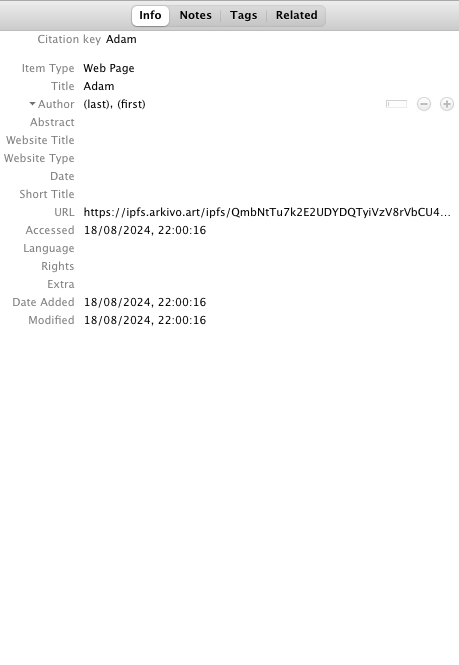
\includegraphics[width=\textwidth]{page-metadata-before.png}
    \caption{Before header metadata}
    \label{fig:image1}
  \end{subfigure}
  \hfill
  \begin{subfigure}[b]{0.45\textwidth}
    \centering
    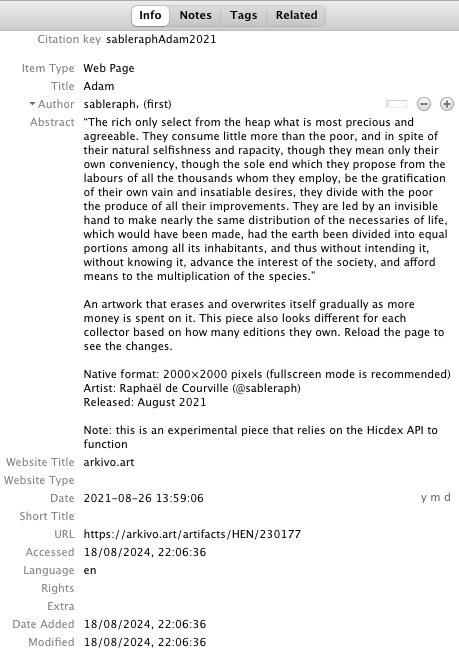
\includegraphics[width=\textwidth]{page-metadata-after.png}
    \caption{After header metadata}
    \label{fig:image2}
  \end{subfigure}
  \caption{Artifact metadata pulled by Zotero}
  \label{fig:zotero-metadata-comparison}
\end{figure}



\subsection{Snapshots}

The first snapshot is important, as it is used for the initial classification of the OBJKT, as well as to establish a baseline record, against which future snapshots can be compared.
Therefore it should be taken immediately after discovery/ingestion.



\subsection{Encapsulation of internal IDs}

In normal circumstances the listing of a model, like Artifact, would include the unique ID of that model as stored in the database, for example: \texttt{/artifacts/45}

However this ID is unique to this instance of the application, and it can vary based on the timing of artifact discovery between other instances.
For this reason it is imperative that none of the internal IDs generated by the database are exposed to the user.

In order to achieve this, all URLs must be generated using only public identifiers which uniquely identify a model, in the case of an artifact: \texttt{blockchain /  smart contract / tokenId}.
This scheme closely follows existing proposals for cross-chain standardisation of identifiers \cite{herzogAssetTypeAsset2020}.

So what would be a URL:

\texttt{/artifacts/2065}

Becomes:

\texttt{/artifacts/tezos/KT1RJ6PbjHpwc3M5rw5s2Nbmefwbuwbdxton/230177}


However this URL is quite verbose. For convenience, since most of our initial artifacts are all on tezos, and on the HEN's OBJKT smart contract we can:

\begin{itemize}
    \item omit the blockchain identifier
    \item use an alias for the smart contract address
\end{itemize}

This strategy allows us to have shorter, but still unique URLs, which do not expose our internal DB IDs.

\texttt{/artifacts/HEN/230177}

Of course, the long-form URL should also work.

\subsection{Infrastructure}

A typical centralised application would be sensible to settle for state-of-the-art deployment platforms like Amazon ACS, DigitalOcean, Heroku, or Microsoft Azure. Not only do these commercial infrastructure solutions offer reliable up-time with fast Internet access, but also a wide range of geographically dispersed data centres across the world for maximum resiliency. It is theoretically possible to deploy a distributed and decentralised (control) solution across these platforms from an application point of view, however at the infrastructure level, the control would be centralised on a small number of industry players, which are an easy target for censorship requests from governments (ref needed).

\subsection{Smart Contracts}

boilerplate text, boilerplate text, boilerplate text, boilerplate text, boilerplate text, boilerplate text, boilerplate text, boilerplate text, boilerplate text, boilerplate text.

\subsection{Authentication}

todo: authentication vs authorisation vs access control

One of the main benefits of web3-style authentication is that it does not require any user credentials stored in the application's database. Since all web3 users have their public keys publicly registered on the blockchain, any user can identify themselves by \emph{connecting} their web3 wallet and signing a custom message provided by the application. This way the application can verify who the user is and that they are in possession of the private key, therefore validating their authentication credentials.

\section{Open Source}

Open sourcing this project was essencial because...

\subsection{Open Source License}

The choice of license...


The choice of license for this project was ... due to...



\section{Security: Detecting and Dealing with Malicious Code}

In this section I will talk about the security aspects of code-base artworks.









\section{Prototype Evaluation}


boilerplate text, boilerplate text, boilerplate text, boilerplate text, boilerplate text, boilerplate text, boilerplate text, boilerplate text, boilerplate text, boilerplate text.

\subsection{System Performance}

boilerplate text, boilerplate text, boilerplate text, boilerplate text, boilerplate text, boilerplate text, boilerplate text, boilerplate text, boilerplate text, boilerplate text.

\subsection{End-user study}


The 'Networked Only' checkbox caused some confusion, as one user assumed it was a filter which should instantly be reflected on the results as one checks or unchecks it. Although not originally intended as an auto-updating filter (actual filters were not implemented) the behaviour of the checkbox was altered, by adding an \texttt{onchange} event which submits the form every time it is checked or unchecked. This results in an experience that is more aligned with the user's expectations, and is a reasonable compromise until a proper filtering system is put in place.















